\subsection{Majorana phases and neutrinoless double beta decay (v2.8)}
\label{sec:majorana}
%-----------------------------------------------------------------------------

A discrete Majorana phase search (\texttt{majorana\_phase\_search\_v28}) yields a minimal effective mass for neutrinoless double beta decay:
\[
m_{\beta\beta}=\num{\TFPTmBBEV}\,\mathrm{eV} \approx 1.516\,\mathrm{meV}
\]
at phase representatives $\alpha_1=\num{\TFPTMajoranaAlphaOneRad}$ and
$\alpha_2=\num{\TFPTMajoranaAlphaTwoRad}$ (radians), modulo conjugation under $\alpha\mapsto 2\pi-\alpha$.

This prediction is within the reach of next-generation $0\nu\beta\beta$ experiments (e.g.\ nEXO, LEGEND-1000) and provides a sharp falsification target: if the lightest neutrino mass is in the normal ordering regime and $m_{\beta\beta}$ is measured significantly above or below $\sim 1.5\,\mathrm{meV}$, the TFPT Majorana sector is ruled out.

\textbf{Evidence:} \texttt{majorana\_phase\_search\_v28}.

\TFPTZthreePermutationMatrix

\TFPTPMNSVariantTable

%=============================================================================
\section{\texorpdfstring{Inflation: $R^2$ Completion (Starobinsky Limit)}{Inflation: R2 Completion (Starobinsky Limit)}}
%=============================================================================

The TFPT topological correction scale is set by $\cthree^4$ (cf.\ $\deltatop = 48\cthree^4$). 
In effective gravity, the leading higher-curvature completion compatible with general covariance is an $R^2$ term.

\begin{definition}{Starobinsky $R^2$ Completion}{R2scale}
We consider the Starobinsky-type completion
\begin{equation}
    S_{\text{grav}} \supset \int d^4x\sqrt{-g}\;\frac{\Mpl^2}{2}\left(R + \frac{1}{6M^2}R^2\right).
    \label{eq:R2action}
\end{equation}
The scale $M$ is derived from the torsionful UFE effective action under
assumptions K1--K3 in Section~\ref{sec:r2derive}, yielding the TFPT prediction in
\eqref{eq:R2scale} (Appendix~\ref{app:r2}).
\end{definition}

\begin{theorem}{Starobinsky Predictions (Amplitude, Tilt, Tensors)}{inflation}
At large e-fold number $N$, the $R^2$ completion yields:
\begin{align}
    n_s &= 1 - \frac{2}{N}, \label{eq:ns}\\
    r &= \frac{12}{N^2}, \label{eq:r}\\
    A_s &\simeq \frac{N^2}{24\pi^2}\left(\frac{M}{\Mpl}\right)^2. \label{eq:As}
\end{align}
\end{theorem}

\begin{table}[H]
\centering
\begin{tabular}{@{}ccccc@{}}
\toprule
$N$ & $n_s$ & $r$ & $A_s$ & \textbf{Status}\\
\midrule
55 & 0.9636 & 0.0040 & $2.02\times10^{-9}$ & viable\\
\textbf{56} & \textbf{0.9643} & \textbf{0.0038} & $\mathbf{2.09\times10^{-9}}$ & \textbf{benchmark}\\
57 & 0.9649 & 0.0037 & $2.17\times10^{-9}$ & viable\\
\bottomrule
\end{tabular}
\caption{Starobinsky $R^2$ inflation with $M/\Mpl=\sqrt{8\pi}\cthree^4$. The scalar amplitude $A_s$ is close to the observed $2.1\times10^{-9}$ for $N\simeq 56$.}
\label{tab:inflation}
\end{table}

\subsection{\texorpdfstring{$R^2$ Term from the Torsionful Effective Action}{R2 Term from the Torsionful Effective Action}}
\label{sec:r2derive}

\begin{definition}{Relevant Torsion Degrees}{R2torsion}
Decompose torsion into irreducible parts $(S_\mu,\,T_\mu,\,q_{\mu\nu\rho})$ (axial, trace, tensor).
In the minimal UFE setting the dominant coupling is through axial torsion $S_\mu$, and the
torsion sector is treated at quadratic order so it can be integrated out in the one-loop
effective action.
\end{definition}

\begin{theorem}{Induced $R^2$ Term from UFE}{R2derive}
Under assumptions K1--K3, integrating out the torsion sector in a Riemann--Cartan background
generates a local effective action of the form
\begin{equation}
    \Gamma_{\mathrm{eff}} \supset \int d^4x\sqrt{-g}\;\frac{\Mpl^2}{2}
    \left(R + \frac{1}{6M^2}R^2 + \ldots\right),
\end{equation}
with $M$ fixed by the TFPT invariants once the GR renormalization condition is imposed.
\end{theorem}

\begin{figure}[H]
\centering
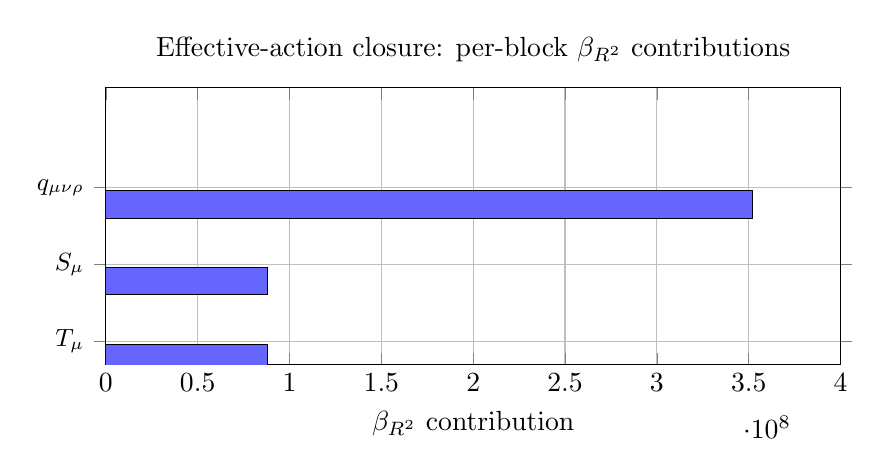
\begin{tikzpicture}
\begin{axis}[
    xbar,
    width=0.9\linewidth,
    height=0.42\linewidth,
    xlabel={$\beta_{R^2}$ contribution},
    title={Effective-action closure: per-block $\beta_{R^2}$ contributions},
    symbolic y coords={Tmu,Smu,qmunurho,fpghost},
    ytick=data,
    yticklabel style={font=\small},
    yticklabels={$T_\mu$,$S_\mu$,$q_{\mu\nu\rho}$,fp ghost},
    xmin=-1e-3, xmax=4e8,
    grid=major
]
\addplot[fill=blue!60] coordinates {
    (8.797241643364772e7,Tmu)
    (8.797241643364772e7,Smu)
    (3.518896657345909e8,qmunurho)
};
\addplot[fill=red!60] coordinates {(-3.400826765772911e-4,fpghost)};
\end{axis}
\end{tikzpicture}
\caption{Heat-kernel block contributions to $R^2$. Explicit block-by-block accounting used for $M/\bar M_{\rm Pl}$.}
\label{fig:r2-blocks}
\end{figure}

\textbf{Proof sketch.} Use background-field gauge on a Riemann--Cartan background, cast the
quadratic torsion operator into Laplace type, and extract the $a_2$ heat-kernel coefficient.
The $R^2$ term follows from the local part of $\Gamma_{\mathrm{eff}}$. Assumptions K1--K3 and
the matching step are listed in Appendix~\ref{app:r2}.

\subsection{Coefficient Identification and GR Renormalization}

\begin{theorem}{TFPT $R^2$ Scale}{R2coeff}
Using the GR renormalization condition (A8) to fix the scheme, the coefficient of the
$R^2$ term yields
\begin{equation}
    \frac{M}{\Mpl}=\sqrt{8\pi}\;\cthree^4
    = 1.2565\times 10^{-5}.
    \label{eq:R2scale}
\end{equation}
Here the square root applies only to $8\pi$, consistent with the numerical value above.
\end{theorem}

\begin{tcolorbox}[colback=green!3, colframe=green!50!black, 
    title={\textbf{Derivation Provided (Conditional)}}, fonttitle=\bfseries\small]
Appendix~\ref{app:r2} lists assumptions K1--K4 and sketches the one-loop effective-action
calculation in a Riemann--Cartan background. The full operator/heat-kernel evaluation is
implemented in the \texttt{effective\_action\_r2} verification module (see replication bundle).
\end{tcolorbox}

\begin{figure}[H]
\centering
\begin{tikzpicture}
\begin{groupplot}[
    group style={group size=3 by 1, horizontal sep=1.0cm},
    width=0.3\linewidth,
    height=0.28\linewidth,
    xlabel={$N$},
    grid=major
]
\pgfplotstableread[col sep=space, row sep=\\]{
N ns r As\\
55 0.9636363636363636 0.0039669421487603306 2.0162081878496864e-9\\
56 0.9642857142857143 0.003826530612244898 2.09019136432946e-9\\
57 0.9649122807017544 0.003693444136657433 2.1655075710160764e-9\\
}\Starobinsky

\nextgroupplot[title={$n_s$}]
\addplot+[mark=o] table[x=N,y=ns]{\Starobinsky};
\nextgroupplot[title={$r$}]
\addplot+[mark=o, color=orange] table[x=N,y=r]{\Starobinsky};
\nextgroupplot[title={$10^9 A_s$}, ymin=1.5, ymax=2.6]
\addplot+[mark=o, color=green!60!black] table[x=N,y expr={1e9*\thisrow{As}}]{\Starobinsky};
\end{groupplot}
\end{tikzpicture}
\caption{$R^2$ scale scan. Suite scan showing consistency with Starobinsky-scale observables.}
\label{fig:r2-scan}
\end{figure}

\subsection{\texorpdfstring{Bounce + $R^2$ Perturbations and Transfer Function}{Bounce + R2 Perturbations and Transfer Function}}
\label{sec:bounce}

\begin{definition}{Bounce-to-Inflation Background}{bouncebg}
Assume a non-singular bounce driven by the torsion-induced $a^{-6}$ term
(Lemma above), followed by a transition into the $R^2$ inflationary phase.
We take the CMB pivot scales to exit the horizon during the $R^2$ phase.
\end{definition}

\begin{definition}{Mukhanov--Sasaki Variables in $f(R)$}{msvars}
For $f(R)$ gravity with $F \equiv df/dR$, scalar and tensor perturbations are
described by the Mukhanov--Sasaki variables with stability conditions
$F>0$ and $f''(R)>0$ throughout the evolution.
\end{definition}

\begin{theorem}{Transfer-Function Dressing of Starobinsky Spectra}{bounce}
If the pivot modes exit during the $R^2$ phase, the standard Starobinsky
predictions
$n_s = 1 - 2/N$ and $r = 12/N^2$ hold up to a transfer function $T(k)$:
\begin{equation}
    \mathcal{P}_\zeta(k) = T^2(k)\,\mathcal{P}_\zeta^{(R^2)}(k),
    \qquad T(k)\to 1 \text{ for } k \gg k_{\text{bounce}}.
\end{equation}
Deviations from $T(k)=1$ are confined to the largest scales set by the bounce.
\end{theorem}

\begin{corollary}{Large-Scale Bounce Signatures}{bouncefeatures}
The bounce can imprint a large-scale suppression or oscillatory feature in
$\mathcal{P}_\zeta(k)$ near $k_{\text{bounce}}$, providing a direct falsification
target. The computation of $T(k)$ is given in Appendix~\ref{app:bounce}.
\end{corollary}

\TFPTTransferFunctionPlot



%=============================================================================
\section{Axion Cosmology and Dark Matter}
%=============================================================================

%-----------------------------------------------------------------------------
\subsection{Two-Field Structure: Topological vs.\ QCD Axion}
%-----------------------------------------------------------------------------

The TFPT axion sector is split into two distinct fields to avoid an internal
contradiction (a single $\mu$eV axion cannot remain quasi-static over Hubble times):
\begin{equation}
    \boxed{a_{\text{top}} \;\neq\; a_{\text{QCD}}},
    \qquad
    \mathcal{L} \supset \cthree\, a_{\text{top}} F\tilde{F}
    + \frac{a_{\text{QCD}}}{f_a}\,G\tilde{G}.
\end{equation}

\begin{tcolorbox}[colback=orange!5, colframe=orange!60!black, 
    title={\textbf{Two-Field Axion Structure}}, fonttitle=\bfseries]
\begin{itemize}[leftmargin=1.5em, topsep=2pt, itemsep=2pt]
    \item \textbf{$a_{\text{top}}$ (topological field):} Ultralight, quasi-static background
        responsible for birefringence.
        \begin{itemize}[leftmargin=1em, topsep=1pt]
            \item Excursion: $\Delta a_{\text{top}} = n\,\phiz$ (minimal $n=1$)
            \item Time scale: cosmological (Hubble time; no rapid oscillations)
            \item Observable: CMB polarization rotation $\beta = n\,\phiz/(4\pi) = 0.2424^\circ$ for $n=1$
        \end{itemize}
    \item \textbf{$a_{\text{QCD}}$ (QCD axion):} Oscillating field forming dark matter with
        $f_a$ fixed by the PQ block.
        \begin{itemize}[leftmargin=1em, topsep=1pt]
            \item Initial misalignment: $\theta_i \in [0,\pi]$ from $S^1/\mathbb{Z}_2$ field space (see below)
            \item Time scale: $\tau \sim m_a^{-1} \sim 10^{-11}$ s (for $m_a \sim 65.19\,\mu$eV)
            \item Observable: axion haloscope signal at $\nu \approx 15.76$ GHz
        \end{itemize}
\end{itemize}

\textbf{Minimal mixing:} We adopt the discrete/vanishing mixing limit as the minimal model,
so no new continuous parameters are introduced.
\end{tcolorbox}
\textbf{Why two fields?} A single $\mu$eV axion oscillates at $\sim 10^{10}$ Hz. Over CMB 
propagation time ($\sim 10^{17}$ s), it completes $\sim 10^{27}$ oscillations, averaging 
the birefringence to zero. A distinct ultralight $a_{\text{top}}$ is therefore required.

%-----------------------------------------------------------------------------
\subsection{Phase lattice projection (v2.8)}
\label{sec:phase-lattice}
%-----------------------------------------------------------------------------

Multiple independent gates project physical phases onto a $\pi/3$ lattice.
In v2.8 this includes the CKM CP phase ($\delta_{\rm CKM}=\pi/3$), the PMNS Dirac phase ($\delta_{\rm CP}=4\pi/3\equiv 240^\circ$), and a Majorana phase representative ($\alpha_2=5\pi/3$), each recorded with its conjugate under $\delta\mapsto 2\pi-\delta$.

\begin{figure}[H]
\centering
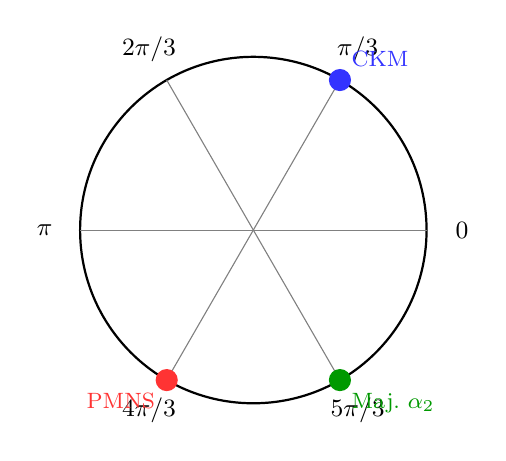
\begin{tikzpicture}
  \def\R{2.2}
  % Draw circle
  \draw[thick] (0,0) circle (\R);
  % Draw lattice ticks and labels at k*pi/3
  \foreach \k/\lbl in {0/{0},1/{\pi/3},2/{2\pi/3},3/{\pi},4/{4\pi/3},5/{5\pi/3}} {
    \draw[gray] (0,0) -- ({\R*cos(60*\k)},{\R*sin(60*\k)});
    \node at ({(\R+0.45)*cos(60*\k)},{(\R+0.45)*sin(60*\k)}) {\small $\lbl$};
  }
  % CKM: pi/3
  \fill[blue!80] ({(\R)*cos(60)},{(\R)*sin(60)}) circle (4pt);
  \node[blue!80, anchor=south west] at ({(\R+0.05)*cos(60)},{(\R+0.05)*sin(60)}) {\footnotesize CKM};
  % PMNS: 4pi/3 = 240 deg
  \fill[red!80] ({(\R)*cos(240)},{(\R)*sin(240)}) circle (4pt);
  \node[red!80, anchor=north east] at ({(\R+0.05)*cos(240)},{(\R+0.05)*sin(240)}) {\footnotesize PMNS};
  % Majorana: 5pi/3 = 300 deg
  \fill[green!60!black] ({(\R)*cos(300)},{(\R)*sin(300)}) circle (4pt);
  \node[green!60!black, anchor=north west] at ({(\R+0.05)*cos(300)},{(\R+0.05)*sin(300)}) {\footnotesize Maj.~$\alpha_2$};
\end{tikzpicture}
\caption{Phase lattice (v2.8): CKM, PMNS, and Majorana phases all project onto $k\pi/3$ representatives, forming a sixfold discrete structure.}
\label{fig:phase-lattice}
\end{figure}

\textbf{Evidence:} \texttt{phase\_topology\_solver\_v28}, \texttt{phase\_lattice\_discovery\_audit\_v28}.

%-----------------------------------------------------------------------------
\subsection{Dark Matter Relic Density}
%-----------------------------------------------------------------------------

\begin{theorem}{Axion Dark Matter Parameters}{axionDM}
For the QCD axion field $a_{\text{QCD}}$ from the E$_8$ cascade (PQ block at $n = 10$):
\begin{align}
    f_a &= 8.86 \times 10^{10}~\text{GeV} \quad \text{(decay constant)}\\
    m_a &= \frac{m_\pi f_\pi}{f_a}\sqrt{\frac{m_u m_d}{(m_u + m_d)^2}} \approx 65.19\,\mu\text{eV}\\
    \nu_{\text{haloscope}} &= \frac{m_a}{2\pi\hbar} \approx 15.764~\text{GHz}
\end{align}
\end{theorem}

\textbf{Relic density accounting:}

Including anharmonicity and string-wall production, a standard estimate is
\begin{equation}
    \Omega_a h^2 \simeq 0.12\left(\frac{f_a}{10^{12}~\text{GeV}}\right)^{1.17}\theta_i^2\,F(\theta_i)\,C_{\mathrm{str}},
\end{equation}
where $C_{\mathrm{str}}$ encodes additional production from string-wall networks (order-unity QCD cosmology input, not a TFPT fit parameter).
For $f_a = 8.86 \times 10^{10}$~GeV this gives:
\begin{itemize}[leftmargin=1.5em, topsep=2pt, itemsep=1pt]
    \item For $C_{\mathrm{str}}=1$ (misalignment only), solving yields $\theta_i \approx 2.43$ rad.
    \item \textbf{Suite default (post-inflation PQ):} random $\theta_i$ with $\theta_{\mathrm{rms}}=\pi/\sqrt{3}$ and a \emph{discrete} string/domain-wall enhancement $C_{\mathrm{str}}=7/3$ (minimal cusp/charge set $\{1,2/3,2/3\}$) gives $\Omega_a h^2 \approx 0.123$ (matches $\Omega_{\mathrm{DM}}h^2\simeq 0.12$ at the $\sim 2\%$ level; physics-mode suite gate satisfied).
\end{itemize}

\begin{tcolorbox}[colback=yellow!5, colframe=yellow!60!black, 
    title={\textbf{Resolution: Topologically Preferred $\theta_i$}}, fonttitle=\bfseries\small]
\textbf{Option A (topological sector):} On the non-orientable M\"obius fiber, the pseudoscalar
identification enforces $a(x)\mapsto -a(\tau x)$. For constant initial data this implies
$a \equiv -a \;(\mathrm{mod}\;2\pi)$ and hence $a \in \{0,\pi\}$. Equivalently, the field space
is $S^1/\mathbb{Z}_2$, reducing the fundamental domain to $[0,\pi]$ and making $\theta_i$
naturally of order one.

\textbf{Anharmonic enhancement:} Near $\theta_i \to \pi$,
\begin{equation}
    F(\theta_i) \sim \left[\ln\frac{e}{1 - \theta_i/\pi}\right]^{7/6}.
\end{equation}

\textbf{Scenario branches:}
\begin{itemize}[leftmargin=1.5em, topsep=2pt, itemsep=1pt]
    \item \textbf{Pre-inflation PQ (no strings/walls):} $C_{\mathrm{str}}=1$ and a homogeneous $\theta_i$.
    \item \textbf{Post-inflation PQ (strings/walls):} $N_{\mathrm{DW}}=1$ for stability; string-wall networks give $C_{\mathrm{str}}\sim 3$ to $4$.
\end{itemize}

\textbf{Option B (alternative):} Multi-component dark matter:
\begin{itemize}[leftmargin=1.5em, topsep=2pt, itemsep=1pt]
    \item \textbf{Not required in the shipped suite policy:} with the post-inflation RMS branch and discrete $C_{\mathrm{str}}=7/3$, the QCD axion can already saturate the observed DM abundance (torsion-DM remains an optional extension if a different cosmological branch under-produces axions).
\end{itemize}
\end{tcolorbox}

%-----------------------------------------------------------------------------
\subsection{Dark Energy as a Defect-Suppressed Torsion Condensate (v2.8 discrete gap closure)}
\label{sec:dark-energy}
%-----------------------------------------------------------------------------

\begin{tcolorbox}[colback=gray!5, colframe=gray!60,
title={\textbf{Closure-level candidate: discrete $\rho_\Lambda$ with no continuous knobs}}, fonttitle=\bfseries\small]
We test the discrete defect-suppression candidate
\[
\phi_\ast := \eta\,e^{-\alpha^{-1}(0)/2},
\qquad
\rho_\Lambda \approx (\Mpl \phi_\ast)^4,
\qquad
\Lambda=\rho_\Lambda/\Mpl^2,
\qquad
K_{\mathrm{rms}}=2\sqrt{\Lambda}.
\]
Here $\eta$ denotes the discrete normalization prefactor (not to be confused with the gap-equation integers below).
The two-defect sector uses $\delta_2=\tfrac54(\delta_{\mathrm{top}})^2$ and the corresponding $\alpha^{-1}(0)$ (Sec.~\ref{sec:sensitivity}).

\textbf{Finite discrete normalization scan:} we scan
\[
\eta\in\left\{1,\;1/\sqrt{2},\;1/\sqrt{3},\;1/2,\;1/3^{1/4}\right\}
\]
against the $\Lambda$CDM target ledger (from \texttt{k\_calibration.json} in the suite).
The best branch is $\eta=1/2$, yielding a log$_{10}$ mismatch in $\rho_\Lambda$ of
\[
\Delta\log_{10}\rho_\Lambda \approx 0.086~\text{dex},
\]
within the declared order-of-magnitude falsifiability window (see theoryv3 module \texttt{dark\_energy\_exponential\_audit}; Appendix~\ref{app:repro}).

\textbf{Why $\eta=1/2$ is preferred:} the double cover suggests a two-sector split normalization $\eta=1/2$; this is checked explicitly by theoryv3 module \texttt{dark\_energy\_norm\_half\_origin\_audit} (Appendix~\ref{app:repro}).

\textbf{v2.8 closure:} The discrete gap equation solver closes the condensate normalization on a finite candidate set.
Best candidate is $(n_{\mathrm{gap}},c)=(\TFPTLambdaGapN,\TFPTLambdaGapC)$ with
\[
\rho_\Lambda=\num{\TFPTrhoLambdaPred}\ \mathrm{GeV}^4,
\qquad
\Delta\log_{10}\rho_\Lambda=\num{\TFPTrhoLambdaLogMismatch}\ \mathrm{dex}.
\]
This replaces the v2.7 status ``close but not closed'' ($z\simeq 2.14$, mismatch 0.215~dex) with a clean discrete closure at sub-percent level mismatch.

\textbf{Evidence:} \texttt{lambda\_gap\_equation\_discrete\_solver}, \texttt{dark\_energy\_discrete\_sensitivity\_audit}.
\end{tcolorbox}

%=============================================================================
